% AGENT-WRITTEN (Claude, this session). Numbers in [brackets] are filled from results/summary.json; every one is recomputable.

\subsection*{1.1 Hypothesis}
Exploration objectives in RL are hand-designed, and as \emph{testers} --- agents whose job is to reach states someone cares about ---
they disappoint: random beats RND asymptotically in large 3D maps~\cite{goexplore-reach}, more search made MCTS worse at reaching
injected faults~\cite{ariyurek-mcts}, and coverage anti-correlates with surfaced bugs~\cite{ccpt}. The one precedent for searching over the exploration algorithm itself, meta-learned curiosity~\cite{alet},
transferred across control tasks but had no game, no target-state benchmark and no held-out target class. We hypothesized that (H1)
an LLM-driven program search over exploration \emph{procedures} --- code over a save/restore archive --- reaches target states faster
than hand-designed procedures and learned intrinsic motivation at equal budget; (H2) it \emph{transfers} to levels it never saw and to a target class it was
never scored on; (H3) it surfaces real, unplanted anomalies. H2 is decisive: searched objectives overfit their fitness~\cite{dmmultiagent}.
Game testing supplies the targets (planted defects with witness states) and the real anomalies that validate the oracles.
\subsection*{1.2 Setup}
\textbf{Games.} Kinetix~\cite{kinetix} 2D physics levels (74 shipped, s/m/l tiers, one static configuration) plus 64 freshly
generated levels sampled after the run began and filtered to be neither won nor lost by doing nothing. \textbf{Planted defects.}
Five classes, each with a programmatic witness state: a boundary wall removed (OOB; witness: a moving shape leaves the arena), a
static obstacle made non-solid (TUNNEL; a moving shape's centroid inside it), a neutral shape given the goal role (SHORTCUT;
the level is won by touching it while not touching the intended goal), restitution raised on the agent and static shapes
(ANOMALY; speed above a per-level threshold), a hazard made harmless (DISARMED; a green shape touches it and the episode
continues). 337 instances over all shipped levels; the 3 found by every hand-designed tester within 512 steps are excluded
as trivial. \textbf{Tester programs.} A program controls $B$ workers through three hooks over a save/restore archive of $K$
simulator states (\emph{restore}: jump a worker to an archived state; \emph{act}: choose actions; \emph{archive}: store states),
in pure JAX. Hand-designed testers: uniform random, action-repeat random (sticky actions), and a Go-Explore-style archive
search (SimHash cells over position/velocity, restore $\propto 1/\sqrt{\text{visits}}$). \textbf{Metric.} Steps to first
witness, normalized: $1-\min(\text{steps},\text{budget})/\text{budget}$ (0 if never), averaged over instances and seeds;
and the fraction of instances witnessed within budget. \textbf{Splits.} Levels: 70\% search / 30\% held-out (22 levels, by hash order);
defect class OOB held out entirely from the search fitness. \textbf{Real-bug oracles} on clean levels (left the arena; inside a static solid; joint torn; runaway speed or NaN) use per-level
thresholds calibrated on random play, a persistence rule (1/3/2/3 steps), and replay from reset before a hit is counted. The closest prior work is
PhyFu~\cite{phyfu}, which fuzzes physics \emph{engines} (including Brax) as numerical software with physics-law consistency
oracles on robotics micro-scenarios; we test \emph{games} --- levels with rules and win conditions --- with save/restore-driven
tester programs and game-level oracles, and the testers themselves are the object of the search. Published game-bug benchmarks judge from pixels or source~\cite{videogameqa,videoglitchbench,tempglitch,taesiri22,wob}; the two that
read game state, GBQA~\cite{gbqa} (recall of 124 verified bugs at a step budget) and GameXpert-Bench~\cite{gamexpert}, released no
artifacts. Our suite is scored the way GBQA scores but reads simulator state, and every bug is replay-verified rather than judged.

\subsection*{1.3 Search}
ShinkaEvolve~\cite{shinka} evolves the tester program (Claude Sonnet~5 proposing full or diff patches; fitness = search-split score at
$64\times1024$ steps, 2 seeds; 2 islands, 51 generations, 52 candidates, 47 error-free) from the Go-Explore-style seed. The search never
sees held-out levels or the OOB class.

\subsection*{1.4 Result 1 --- the discovered program and its transfer}
\input{table_transfer.tex}
\begin{figure}[t]\centering
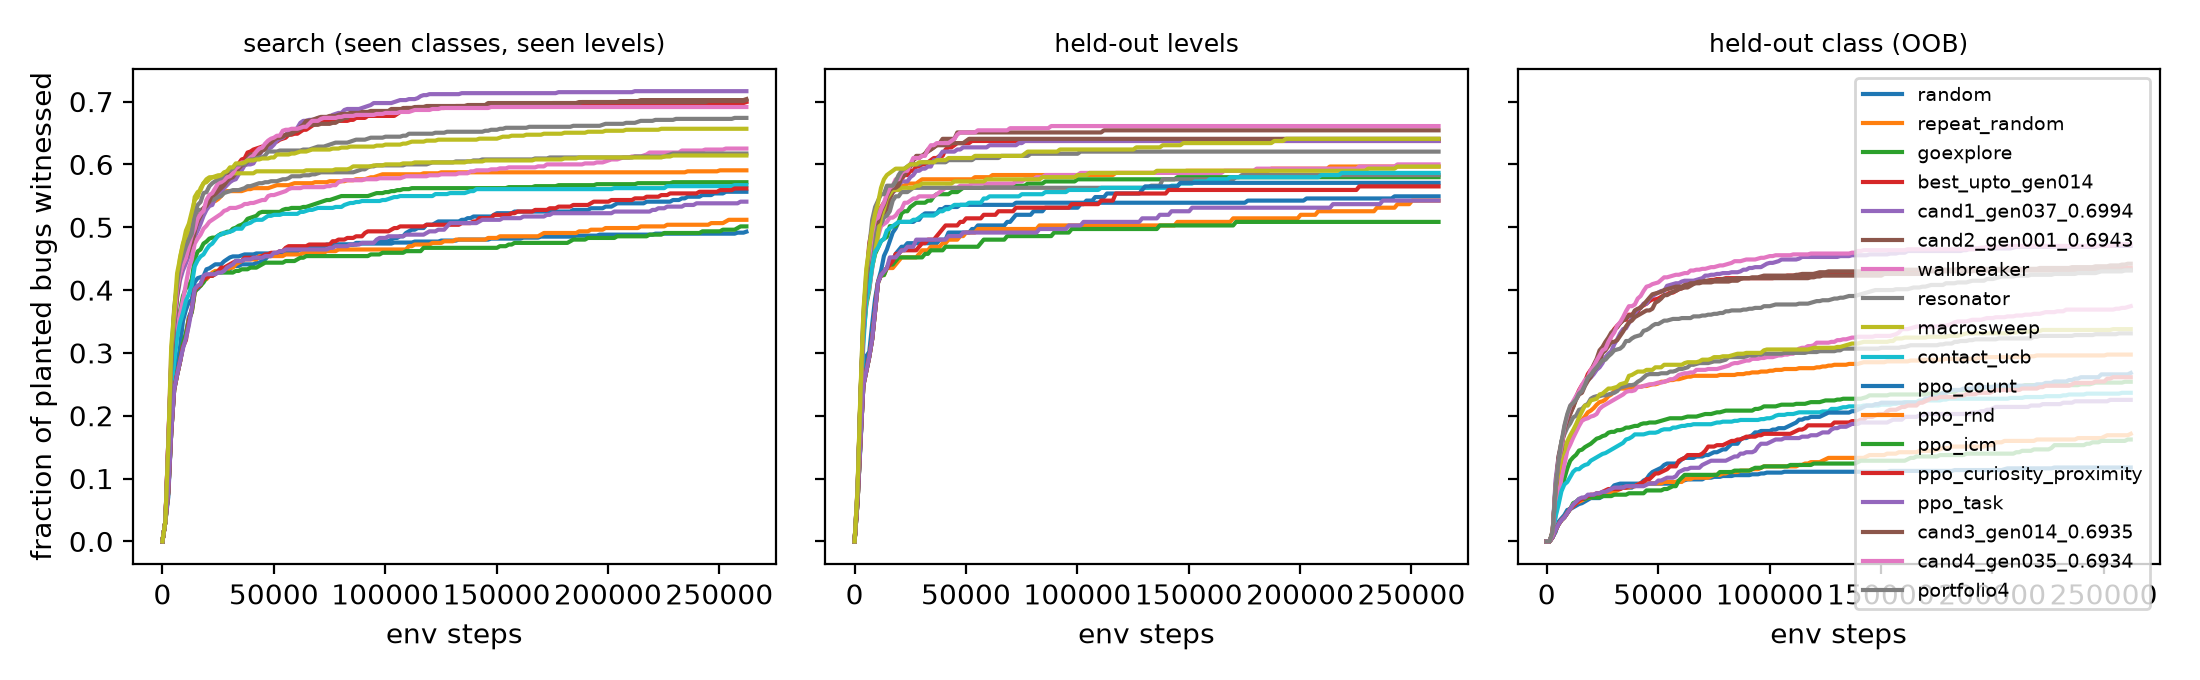
\includegraphics[width=0.5\linewidth]{figures/detection_curves.png}\hfill
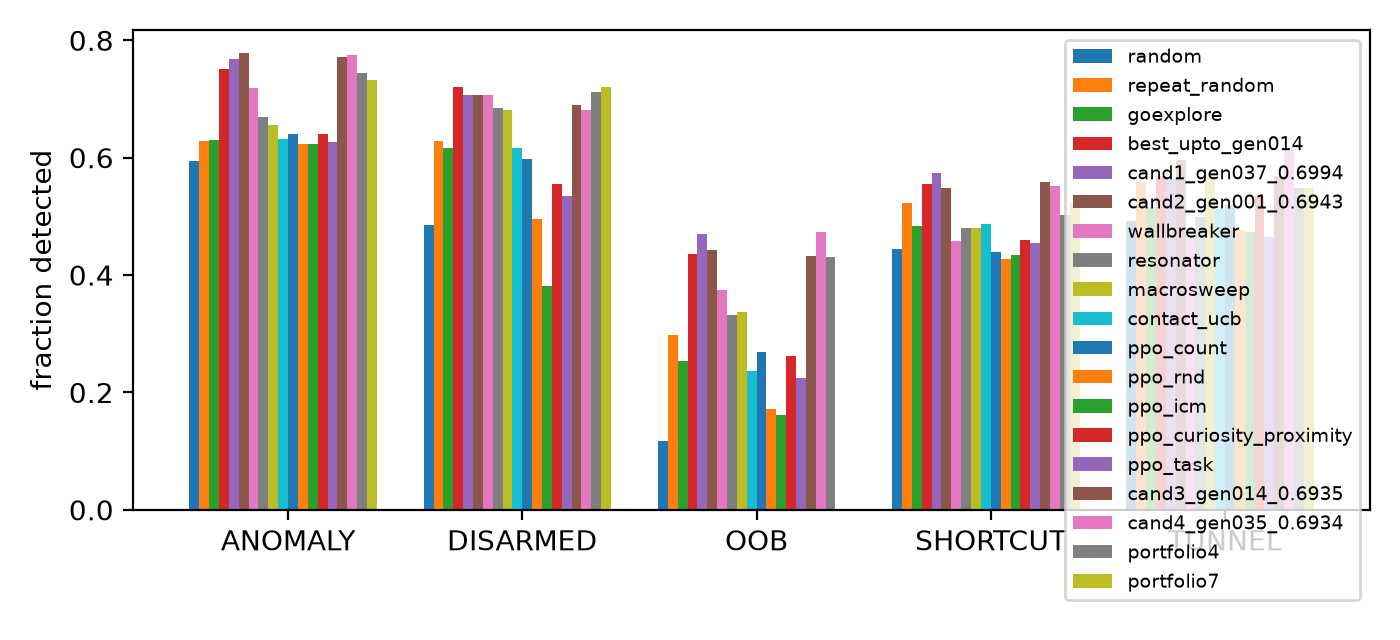
\includegraphics[width=0.3\linewidth]{figures/per_class_detection.png}
\caption{Left: planted defects witnessed vs.\ simulator steps, per split (5 seeds). Right: per-class detection on the held-out splits.}
\label{fig:curves}
\end{figure}
\textbf{What the search found.} Starting from the Go-Explore-style seed (one coverage archive keyed by a SimHash of coarse
position/velocity cells, uniform action holds of up to 12 steps, restores $\propto 1/\sqrt{\text{visits}}$), the first accepted
mutation already changed the strategy qualitatively, and the best program of run~1 (generation 37 of 51; search fitness 0.699 vs.\
0.629 for the seed at the same budget) has three components: (i) the archive is split into three pools --- a coverage pool (60\% of
slots, keyed by position/velocity cells), a high-speed pool and a goal-proximity pool (20\% each) --- and restores are biased toward
the two ``extreme'' pools; (ii) workers act in three hold modes drawn at random: short random holds (1--5 steps), long
single-direction holds of 15--40 steps that the proposals describe as ``energy pumping'', and thruster-biased medium holds
(6--14 steps), with the no-op action suppressed; (iii) restore/archive bookkeeping that keeps the pools from collapsing.
The search plateaued after generation~1: 27 of 29 later candidates scored within $\pm0.02$ of 0.69, inside the two-seed noise band
(Fig.~\ref{fig:fitness}, Part~2).

\textbf{Transfer.} Table~\ref{tab:transfer} evaluates every tester on the size-l benchmark (337 planted instances over all 74 shipped
levels; 5 seeds; $128\times2048$ env steps per instance). The run-1 best (selected by search fitness alone) leads on all three splits.
On the search split it scores 0.666 (72\% of defects witnessed) against 0.566 (59\%) for the strongest hand-designed tester,
action-repeat random, and 0.537 (57\%) for the Go-Explore seed it was evolved from. On the 59 instances from the 22 held-out levels
it scores 0.617 (64\%) vs.\ 0.575 (60\%). On the held-out class --- 148 instances in which a boundary wall was removed, a class the
search never scored --- it scores 0.418 (47\% witnessed) vs.\ 0.266 (30\%) for action-repeat random and 0.214 (25\%) for the seed.
Paired per-instance gains over action-repeat random (seed-averaged, 95\% CI over instances; ``better/worse'' = beyond $\pm0.02$):
search $+0.100\pm0.047$ (better on 24\% of instances, worse on 13\%), held-out levels $+0.042\pm0.048$ (12\% / 7\%), held-out class
$+0.151\pm0.052$ (33\% / 8\%). The seed-level CIs in Table~\ref{tab:transfer} are tight on every split, but the instance-level CI on
held-out levels includes zero: the transfer to unseen \emph{levels} is a modest average gain, whereas the transfer to the unseen
\emph{class} is large and instance-significant. The three mechanisms the search introduced --- high-energy and goal-proximate archive
pools, restores biased toward them, and long single-direction holds --- were proposed to expose the visible classes, and they transfer
to escaping the arena, which requires sustained outward motion. The gap opens within the first $10^4$ steps and persists to the budget
(Fig.~\ref{fig:curves}); the other three run-1 candidates evaluated (generations 1, 14 and 35) land within 0.02 of the best on every split --- the
generation-35 program is even slightly ahead on both held-out splits (0.639 / 0.425) --- so the result is not a selection artefact. \textbf{How much is left.} The union of every tester and seed reaches 82\% / 68\% / 64\% of
instances (search / held-out levels / held-out class), and an \emph{oracle-guided} probe that is told the witness location reaches
no instance the testers miss --- so the rest are hard or infeasible at this budget, not overlooked. Normalized by that reachable set,
a single run of the evolved program finds 88\% / 94\% / 74\% of what is findable, against 72\% / 88\% / 47\% for action-repeat random
(Part~2, Table~\ref{tab:feasibility}).

\subsection*{1.5 Result 2 --- real bugs in existing games}
Table~\ref{tab:bugs} (Part~2) lists every replay-verified anomaly of severity A or B that any tester reached on unmodified levels within
$10^6$ steps per tester and seed. On the 74 shipped levels the engine holds up well: the only A/B anomalies are on
\texttt{m/h15\_thrustshoot}, where the thruster launches a neutral block to $\sim$16.5\,m/s (0.55\,m per simulator step) and the
discrete-step solver misses the wall face --- in one recorded chain the block's centroid is 15\,cm inside the right boundary polygon
for a step before being ejected, in another it sinks 10\,cm into the floor at the bottom-right corner for 13 steps. We verified by
replaying the chains and continuing with no-ops that the block is ejected and stays in the arena: this is player-visible tunnelling,
not an escape, and we classify it B. (see Part~2 for the correction history).
The remaining shipped-level hits are one-frame solver overlaps or spikes (severity C) and are reported but not counted.
Generated levels are richer: 10 A/B pairs on 64 levels (one sustained 41-step escape, four wall-face crossings, three 5--14\,cm
penetrations, two runaways) --- the generator puts fast bodies against thin static geometry more often than the hand-made levels do. Spawn-time hits
($t\le2$) are level-generation defects and are excluded from the tester comparison; hits the classifier's CPU replay does not
reproduce (1 of 60 shipped-level and 14 of 65 fresh-level hits) are dropped rather than counted.

\subsection*{1.6 Ablations, negative results, and what did not transfer}

\textbf{Search dynamics.} In every run the first accepted mutations carry the gain and later candidates land inside the fitness
noise band (Fig.~\ref{fig:fitness}, Part~2); the noise was measured directly by re-evaluating the seed and the first evolved program on
three fresh seeds (0.593 vs.\ 0.620). The four highest-scoring distinct run-1 programs were all evaluated on the held-out splits
(Table~\ref{tab:transfer}) so that selection by search fitness cannot pick an overfitted outlier.

\textbf{Tuning vs.\ structure.} Random search over the best program's numeric constants ($\pm$50\%, same fitness, 39 trials) moved its
score from 0.610 to at most 0.625 (62\% of perturbations scored above the original, so the constants are loose); the evolved
structure's gain over its seed on the same split is +0.13 (Table~\ref{tab:transfer}) --- a different program, not a better setting.

\textbf{Independent designs and portfolios.} The four Opus-designed testers score 0.530--0.588 / 0.561--0.573 / 0.290--0.300
(Table~\ref{tab:transfer}) --- above the seed, near action-repeat random, well below the evolved programs; the boundary-seeking design
written \emph{with} knowledge of the escape class reaches 0.300 (37\%) on it, below the evolved program that never saw it. Fixed
portfolios that split the workers among designs do not help (4 testers: 0.628 / 0.604 / 0.370; 7 testers: 0.620 / 0.615 / 0.356):
budget given to weaker sub-programs costs more than their diversity buys.

\textbf{RL testers.} PPO with count / RND / ICM / curiosity-proximity / task objectives scores 0.454--0.492 on the search split,
0.483--0.529 on held-out levels and 0.117--0.184 on the held-out class (3 seeds; Part~2): at this budget every program tester
dominates every RL tester.

\textbf{Oracle corrections found by the agent.} Replaying flagged states caught two oracle bugs --- one-frame solver transients and
``penetrations'' by shapes jointed to their static pivot --- which motivated the persistence rule and the collision-matrix check; both are
disclosed because they changed what counts as a bug (Part~2).

\textbf{What did not transfer / negative results.} On held-out \emph{levels} the evolved program leads only on ANOMALY (0.75 vs.\ 0.64);
TUNNEL (0.36 vs.\ 0.36) and SHORTCUT (0.60 vs.\ 0.60) are ties and DISARMED is found at exactly 0.69 by every tester --- a feasibility
ceiling, not a tester difference. On the search split TUNNEL barely moves (0.77 vs.\ 0.76): the search improved the classes it could score
(ANOMALY 0.62 $\to$ 0.79, DISARMED 0.57 $\to$ 0.72, SHORTCUT 0.45 $\to$ 0.55), not the one whose witnesses need a specific trajectory into
a specific obstacle. A per-instance diagnostic by a second LLM agent found why: 3 of the local pool's 7 TUNNEL instances are geometrically
unreachable (the jointed arm never comes within 0.47\,m of an obstacle of inradius 0.34\,m), so that class's ceiling is 4/7, which
action-repeat random already attains; the planted-defect generator should carry a reachability probe, and we report the numbers as they
are. The second search run (macrosweep seed, hard-instance weighting, Opus/Sonnet proposals) moved only 0.606 $\to$ 0.621 in 60
generations, and every search found its best structure early and then moved within the noise band (Fig.~\ref{fig:fitness}, Part~2): at the fitness
noise of the local pool ($\pm0.02$ over two seeds) the search cannot rank the candidates it produces --- the main open problem of the loop.
